\documentclass[12pt]{article}

\input{preambulo.tex}
\input{portada.tex}

\usepackage{booktabs}
\usepackage{multirow}
\usepackage{listings}
\usepackage{xcolor}
\usepackage{subcaption}

% Definición de colores pastel y modernos
\definecolor{backcolour}{rgb}{0.96,0.96,0.96}
\definecolor{codegreen}{rgb}{0.13,0.55,0.13}
\definecolor{codegray}{rgb}{0.5,0.5,0.5}
\definecolor{codepurple}{rgb}{0.58,0,0.82}
\definecolor{codeblue}{rgb}{0.0,0.0,0.8}

% Configuración del estilo moderno
\lstdefinestyle{modern}{
    backgroundcolor=\color{backcolour},   
    commentstyle=\color{codegreen}\itshape,
    keywordstyle=\color{codeblue}\bfseries,
    numberstyle=\tiny\color{codegray},
    stringstyle=\color{codepurple},
    basicstyle=\ttfamily\scriptsize,
    breakatwhitespace=false,         
    breaklines=true,                 
    captionpos=b,                    
    keepspaces=true,                 
    numbers=left,                    
    numbersep=10pt,                  
    showspaces=false,                
    showstringspaces=false,
    showtabs=false,                  
    tabsize=4,
    frame=single,                    % Marco simple alrededor del código
    rulecolor=\color{lightgray},     % Color del marco
    xleftmargin=15pt,                % Margen para que los números no se peguen
    literate={á}{{\'a}}1 {é}{{\'e}}1 {í}{{\'i}}1 {ó}{{\'o}}1 {ú}{{\'u}}1
             {Á}{{\'A}}1 {É}{{\'E}}1 {Í}{{\'I}}1 {Ó}{{\'O}}1 {Ú}{{\'U}}1
             {ñ}{{\~n}}1 {Ñ}{{\~N}}1
}

% Aplicar el estilo por defecto a todos los bloques de código
\lstset{style=modern}

\begin{document}
    \portada[%
        titulo=Metaheurísticas,
        subtitulo=Práctica 1:\\ Técnicas de Búsqueda de Poblaciones para el Problema de Asignación Con Restricciones (PAR),
        autor=Jesús Muñoz Velasco,
        dni=76668409W,
        email=jesusmuve18@correo.ugr.es,
        horario practicas=Miércoles 15:30 - 17:30 (Grupo A3),
        año=Curso 2025-2026]
        
    \thispagestyle{empty}
    \tableofcontents
    \newpage
    \thispagestyle{empty}

    \section{Descripción del problema}

    El Problema de Agrupamiento con Restricciones (PAR), también conocido como \textit{Constrained Clustering}, consiste en la partición de un conjunto de $n$ datos o instancias en $k$ grupos (clústeres) disjuntos, basándose en la similitud de sus características y cumpliendo en la mayor medida posible un conjunto de restricciones impuestas sobre los pares de instancias. \\
    
    Formalmente, sea $X = \{x_1, x_2, \dots, x_n\}$ un conjunto de $n$ elementos en un espacio de dimensión $d$. El objetivo es encontrar una partición $C = \{C_1, C_2, \dots, C_k\}$ tal que se minimice la dispersión intra-clúster (medida como la distancia euclídea de cada elemento al centroide de su clúster), sujeta a un conjunto de restricciones a nivel de instancia (de tipo Must-Link y Cannot-Link). \\
    
    Hay 2 tipos de restricciones posibles sobre 2 instancias $x_i,x_j\in X$:
    \begin{itemize}
        \item \textit{Must-Link} (ML). Los elementos $x_i$ y $x_j$ deben pertenecer al mismo clúster.
        \item \textit{Cannot-Link} (CL). Los elementos $x_i$ y $x_j$ no pueden pertenecer al mismo clúster.
    \end{itemize}
    
    Dado que encontrar una solución factible que satisfaga todas las restricciones es un problema NP-completo en la mayoría de configuraciones prácticas, relajaremos el incumplimiento de estas condiciones, donde las violaciones se penalizan en la función objetivo. La función objetivo a minimizar se define como
    \begin{gather*}
        fitness(solucion) = desviacion(solucion) + \lambda \cdot infeasibility(solucion)
    \end{gather*}
    donde establecemos $\lambda = \frac{max_ {dist}(X)}{restricciones(R)}$ para asegurar que la infactibilidad y la desviación tienen la suficiente relevancia. Además, la desviación de una solución se define como 
    \begin{gather*}
        desviacion(C_s) = \frac{1}{k} \sum_{C_i\in C_s} \frac{1}{|C_i|} \sum_{\vec{x_j}\in C_i} \left\|\vec{x_j} - \frac{1}{|C_i|} \sum_{x_j\in C_i} \vec{X_j}\right\|
    \end{gather*}
    y la infactibilidad como el número de condiciciones inclumplidas de una solución.

    \newpage

    \section{Aplicación de los algoritmos empleados}

    Para la resolución del PAR mediante los algoritmos Aleatorio, Greedy y Búsqueda Local, es necesario establecer un marco de trabajo común que defina cómo se representan, evalúan y manipulan las soluciones.

    \subsection{Esquema de representación de soluciones}
    Una solución $S$ se representa como un vector de tamaño $n$ (número de instancias), donde el índice $i$ representa la instancia $x_i$, y el valor almacenado en $S[i]$ indica el índice del clúster al que ha sido asignada.
    \begin{gather*}
        S = [c_0, c_1, \dots, c_{n-1}] \quad \text{donde} \quad c_i \in \{0,1, \dots, k-1\}
    \end{gather*}
    Esta representación garantiza que toda instancia pertenezca a un clúster y solo uno. 

    \subsection{Esquema de representación de restricciones}
    Para representar el conjunto de restricciones $R$ se pueden usar dos estrategias principalmente, según convenga para mayor eficiencia en las evaluaciones de una solución:
    \subsubsection{Forma Matricial}
    El conjunto $R$ se representa como una matriz de dimensión $n\times n$ donde cada elemento $R_{ij}$ representará la restricción existente entre la instancia $x_i$ y la $x_j$. Podrá tomar los siguientes valores:
    \begin{itemize}
        \item $R_{ij} = 1$: Indica una restricción \textit{Must-Link}.
        \item $R_{ij} = -1$: Indica una restricción \textit{Cannot-Link}.
        \item $R_{ij} = 0$: Indica que no existe ninguna restricción entre $x_i$ y $x_j$.
    \end{itemize}
    Por la naturaleza de esta matriz será cuadrada, simétrica y los elementos de la diagonal principal no podrán valer $-1$. Es muy útil para saber si 2 elementos tienen alguna restricción entre ellos.

    \subsubsection{Forma Vectorial}
    En este caso se ha creado un nuevo tipo de dato llamado ``Restricción'' y tendrá la siguiente estructura:

\begin{lstlisting}[language=C++,mathescape=true, caption={Estructura de una restricción vectorial}, label={lst:VresStructure}]
struct Restriccion:
    i,j       // Indices de los puntos $x_i$ y $x_j$ que participan en la restricción
    tipo      // 1 para Must-Link, -1 para Cannot-Link
\end{lstlisting}
    De esta forma, el conjunto de restricciones $R$ será un vector de ``Restricciones'' según acabamos de describir. Aunque esta estructura sea peor para saber si 2 elementos tienen alguna restricción, es mucho mejor para recorrer las restricciones una por una para cálculos como la infactibilidad.

    \subsection{Criterio de validación de Soluciones}
    Dado que el problema establece que hay un número $k$ de clústeres para la solución se considerará que una solución $S$ es válida si y solo si aparecen todos los clústeres en la solución, es decir, si se verifica que 
    \begin{gather*}
        c_i\in S \ \ \ \ \forall c_i\in \{0,1,...,k-1\} 
    \end{gather*}

    \subsection{Reparación de soluciones no válidas}
    El proceso de reparación de una solución $S$ con clústeres vacíos consistirá en seleccionar un elemento $c_0\in S$ que aparezca al menos 2 veces en el vector (para no dejar dicho clúster vacío) y sustituir su valor por el índice del clúster vacío. Se repite este proceso hasta que no haya clústeres vacíos. Seguiría el siguiente esquema:

\begin{lstlisting}[language=C++,mathescape=true, caption={Pseudocódigo de la reparación de una solución}, label={lst:fixSolution}]
Función RepararSolucion(S):
    // Inicializamos el vector n_puntos con el número de puntos de cada clúster en la solucion S
    n_puntos = nPuntosClusteres(S)

    Para cada clúster c desde 0 hasta $k-1$:
        Si n_puntos[c] == 0:
            arreglado = Falso
            instancia = 1
            
            // Buscar una instancia de un clúster con más de 1 elemento
            Mientras arreglado == Falso y instancia $\leq$ n:
                cluster_actual = S[instancia]
                
                Si n_puntos[cluster_actual] > 1:
                    // Reasignar al clúster vacío
                    S[instancia] = c_vacio       
                    n_puntos[cluster_actual] = n_puntos[cluster_actual] - 1
                    n_puntos[c_vacio] = n_puntos[c_vacio] + 1
                    arreglado = Verdadero

                instancia++

    return S
\end{lstlisting}
    
    \subsection{Evaluación de una solución (función objetivo)}
    La evaluación de una solución requiere calcular los centroides de los clústeres a partir de las asignaciones actuales en $S$, calcular la desviación media de cada clúster y contabilizar las restricciones violadas consultando la matriz $R$. Esto se hará de la siguiente forma:
    
    \subsubsection{Cálculo de centroides de una solución}

\begin{lstlisting}[language=C++, mathescape=true, caption={Pseudocódigo del cálculo de los centroides de una solución}, label={lst:getcentroids}]
Funcion obtenerCentroides(S):
    n_puntos = nPuntosClusteres(S)

    // Recorro todos los vectores sumándolos a su cluster
    Para cada instancia i de X:
        cluster = S[i]
        Para cada dimension d de la instancia i:
            centroides[cluster].coordenada[d] += X[i].coordenada[d]
    

    // Divido entre el número de cada cluster para calcular la media
    Para cada cluster c desde 0 hasta $k-1$
        Para cada dimension d del centroide centroides[c]:
            centroides[c].coordenada[d] /= n_puntos[c]

    return centroides
\end{lstlisting}

    \subsubsection{Cálculo la desviación de una solución}
    
\begin{lstlisting}[language=C++, mathescape=true, caption={Pseudocódigo del cálculo de la desviación de una solución}, label={lst:desviation}]
Función Desviacion(S):
    centroides = obtenerCentroides(S)
    n_puntos = nPuntosClusteres(S)

    // Sumamos las distancias
    Para cada instancia i de X:
        cluster = S[i]
        $distancia_{ic}$[cluster] += distancia(X[i], centroides[cluster])

    desviacion = 0

    // Sumamos la media de las distancias
    Para cada clúster c desde 0 hasta $k-1$
        Si n_puntos[c] > 0:
            desviacion += ($distancia_{ic}$[c]/n)

    return (desviacion/k)
\end{lstlisting}

    \subsubsection{Cálculo la infactibilidad de una solución}
    
\begin{lstlisting}[language=C++, mathescape=true, caption={Pseudocódigo del cálculo de la infactibilidad de una solución}, label={lst:infeasibility}]
Función Infactibilidad(S):
    inf = 0

    Para cada restricción res en el conjunto de restricciones R
        juntos = (S[res.i] == S[res.j])

        Si res es de tipo ML y !juntos:
            inf++ // Error: Deberían estar juntos (Must-Link)
        Sino si res es de tipo CL y juntos:
            inf++ // Error: No deberían estar juntos (Cannot-Link)
    
    return inf
\end{lstlisting}

    \subsubsection{Evaluación de una solución}
    Finalmente, usando las funciones previamente descritas, y previamente fijado el valor de lambda, la función objetivo se calculará de la siguiente forma
\begin{lstlisting}[language=C++, mathescape=true, caption={Pseudocódigo del cálculo de la función objetivo}, label={lst:infeasibility}]
Evaluacion(S) {
        C = Desviacion(S)
        inf = Infactibilidad(S)

        return (C + lambda * inf)
    }
\end{lstlisting}

    \newpage

    \section{Estructura del método de búsqueda}
    A continuación se describen más a fondo cada algoritmo utilizado junto con una descripción de las funciones propias que estos usan. 

    \subsection{Algoritmo aleatorio}

    El algoritmo aleatorio genera múltiples soluciones independientes, evalúa cada una usando la función objetivo descrita previamente, y devuelve la mejor encontrada tras un número determinado de iteraciones. El código sigue la siguiente estructura:

\begin{lstlisting}[language=C++,mathescape=true, caption={Estructura del algoritmo aleatorio}, label={lst:VresStructure}]
optimizarAleatorio(maxevals):
    mejor_fitness = -1
    mejor_solucion = null

    Para cada iteracion i desde 0 hasta maxevals:
      S = generarSolucionAleatoria()
      fitness = Evaluacion(S)

      Si fitness < mejor_fitness o mejor_fitness < 0: 
        mejor_solucion = S
        mejor_fitness = fitness
      
    return mejor_solucion
\end{lstlisting}

    \subsection{Algoritmo Greedy}
    El algoritmo Greedy construye la solución paso a paso. Comienza con una solución generada aleatoriamente. Comienza generando una solución aleatoria que sea válida (si no lo es se arregla como se ha descrito en la sección anterior). Posteriormente se realiza un proceso iterativo en el que se prueba a modificar la solución anterior probando en cada punto del vector solución qué ocurriría al asignarlo a cada clúster. De entre estas modificaciones virtuales se elegirá aquella que minimice el número de restricciones incumplidas y en caso de empate se elegirá la que minimice la desviación general. Este proceso se realizará hasta que no se encuentre una configuración mejor modificando un único elemento.

    \subsubsection{Función Heurística (Incremento del coste)}
    La heurística en este caso valora el coste de añadir la instancia $x_i$ al clúster $c$. Se calcula la distancia al centroide actual del clúster y las penalizaciones por restricciones generadas con las instancias ya asignadas (función evaluación anterior). 
    
    % Además, en este caso para optimizar el cálculo, en lugar de realizar este cálculo como se ha desarrollado se valorará solo las modificaciones que implica cambiar un único elemento de clúster, ya que esto solo cambia el cálculo de la desviación y la infactibilidad de 2 clúster (el anterior y el nuevo asignado a la instancia $x_i$). Esto se calculará de la siguiente forma:

    \subsubsection{Estructura del código Greedy}
    Con la heurística ya mencionada, el algoritmo seguirá la siguiente estructura

\begin{lstlisting}[language=C++,mathescape=true, caption={Estructura del algoritmo Greedy}, label={lst:greedy}]
optimizarGreedy(maxevals):
    
    // Generamos aleatoriamente centroides en el dominio del problema
    centroides = generarCentroidesAleatorios()

    // Generamos una solución aleatoria
    S = generarSolucionAleatoria()

    Si S no es válida:
        S = RepararSolucion(S)

    // Generamos y barajamos los índices
    RSI = generarIndices(0,n-1)
    barajar(RSI)

    Repetir:
        modificado = false

        Para cada índice i de RSI:
            cluster_actual = S[i]
            mejor_cluster = currentCluster
            mejor_inf = infinito
            mejor_d = infinito

            // Evaluar todos los posibles clústeres para el punto $x_i$
            Para cada indice j desde 0 hasta k-1:
                inf = Evaluacion(S)
                d = ditancia(X[i], centroides[j])

                Si inf < mejor_inf:
                    mejor_inf = inf
                    mejor_d = d
                    mejor_cluster = j
                Sino si inf == mejor_inf y d < mejor_d:
                    mejor_d = d
                    mejor_cluster = j

            // Si hay un clúster mejor para este punto
            Si mejor_cluster != cluster_actual:
                S[i] = mejor_cluster
                modificado = true

    Mientras modificado==true

    return S
\end{lstlisting}

    \subsection{Algoritmo de Búsqueda Local}

    El algoritmo de Búsqueda Local parte de una solución inicial (generada aleatoriamente) y explora su vecindario aplicando pequeñas modificaciones. Si un vecino mejora la función objetivo, reemplaza a la solución actual. El proceso se detiene cuando ningún vecino mejora la solución (óptimo local) o se alcanza el límite de evaluaciones. Para ello se sirve de las siguientes funciones:

    \subsubsection{Generación del vecindario}
    Dada una solución $S$, se genera su vecindario, entendiendo este como los cambios posibles de clúster, que serán factibles siempre y cuando cumplan con no dejar un clúster vacío. Se hará de la siguiente forma:

\begin{lstlisting}[language=C++,mathescape=true, caption={Pseudocódigo de la generación del vecindario}, label={lst:greedy}]
generarVecindario(S):
    Para cada i desde 0 hasta n-1:
        cluster_actual = S[i]
            
        // Sólo guardamos los factibles
        Si nPuntosCluster(cluster_actual) > 1:
            Para cada indice j desde 0 hasta k-1:
                Si j!=cluster_actual:
                    vecindario.añadir({i, j})

    return vecindario
\end{lstlisting}

    \subsubsection{Factorización de la solución}
Dado que evaluar la función objetivo completa tiene un coste computacional alto se implementa una factorización de la solución donde se tienen precalculados ciertos valores. Al mover $x_i$ del $c_{origen}$ al $c_{destino}$ tan solo se producen cambios en estos 2 clústeres por lo que solo habrá que comprobar si con este nuevo cambio se incumple alguna restricción o si se ha dejado de incumplir una que existía previamente. Para la distancia tan solo se tendrá que recalcular la dispersión media de estos 2 clústeres y reconsiderar la suma de todos. Para que esto sea posible se genera una estructura como la siguiente:

\begin{lstlisting}[language=C++,mathescape=true, caption={Pseudocódigo de la generación del vecindario}, label={lst:greedy}]
Clase factorizacionSolucion:
    infactibilidad                      // Número de restricciones incumplidas
    centroides                          // Vector de centroides actuales
    n_puntos_cluster                   // Vector de número de puntos por cluster
    distancia_ic                        // Vector de distancia intra-cluster
    desviacionGeneral                   // Desviación general     
    fitness                             // Función fitness     
\end{lstlisting}

    De esta forma, si se inicializa adecuadamente, la actualización de una solución tras asignar $x_i$ al nuevo cluster $c_{nuevo}$ quedaría de la siguiente forma:
\begin{lstlisting}[language=C++,mathescape=true, caption={Pseudocódigo de la actualización de una solución factorizada}, label={lst:greedy}]
funcion ActualizarFactorizacionSolucion(S, S_fac, i, c_nuevo):
    c_anterior = S[i]
    Si c_anterior == c_nuevo:
        return S_fac   // Si no cambia de cluster, no hacemos nada

// Actualizamos infeasibility
    S_fac.infactibilidad = ActualizarInfactibilidad(S, S_fac, i, c_nuevo)

// Actualizamos centroides
    n_anterior = S_info.n_puntos_cluster[c_anterior]
    n_nuevo = S_info.n_puntos_cluster[c_nuevo]

    // Extraemos el punto del centroide anterior: (Media_anterior * N - Punto) / (N - 1)
    Para cada d desde 0 hasta la dimensión de X[i]:
        suma_anterior = S_fac.centroides[c_anterior].coordenada[d] * n_anterior
        S_info.centroides[c_anterior].coordenada[d] = (suma_anterior - X[i].coordenada[d]) / (n_anterior - 1);

    // Añadimos el punto al centroide nuevo: (Media_vieja * N + Punto) / (N + 1)
    Para cada d desde 0 hasta la dimensión de X[i]:
        suma_anterior = S_fac.centroides[c_nuevo].coordenada[d] * n_nuevo
        S_info.centroides[c_nuevo].coordenada[d] = (suma_anterior + X[i].coordenada[d]) / (n_nuevo - 1);

// Actualizamos la cantidad de puntos
    S_fac.n_puntos_cluster[c_anterior]--
    S_fac.n_puntos_cluster[c_nuevo]++

// Actualizamos la distancia intra-cluster
    // Como el centroide se movió, recalculamos las distancias solo de los puntos en c_anterior y c_nuevo
    anterior_dist_ic_anterior = S_fac.distancia_ic[c_anterior]
    anterior_dist_ic_nueva = S_fac.distancia_ic[c_nuevo]
    
    nueva_dist_ic_anterior = 0.0
    nueva_dist_ic_nueva = 0.0

    Para cada j desde 0 hasta n-1:
        Si j==i:
            // El punto que se mueve, ahora se mide respecto a c_nuevo
            nueva_dist_ic_nueva += distancia(X[i], S_fac.centroides[c_nuevo])
        Sino si S[j] == c_anterior:
            nueva_dist_ic_anterior += distancia(X[i], S_fac.centroides[c_anterior])
        Sino si S[j] =0 c_nueva:
            nueva_dist_ic_nueva += distancia(X[j], S_fac.centroides[c_nuevo])

    S_fac.distancia_ic[c_anterior] = nueva_dist_ic_anterior
    S_fac.distancia_ic[c_nuevo] = nueva_dist_ic_nueva

// Actualizamos la desviación general
    // Media antigua de estos dos clústeres
    anterior_contrib_anterior = Si (n_anterior > 0) entonces (anterior_dist_ic_anterior / n_anterior) Sino 0.0
    anterior_contrib_nueva = Si (n_nuevo > 0) entonces (anterior_dist_ic_nueva / n_nuevo) Sino 0.0

    // Media nueva de estos dos clústeres
    nuevo_n_anterior = S_fac.n_puntos_cluster[c_anterior];
    nuevo_n_nuevo = S_fac.n_puntos_cluster[c_nuevo];
    nueva_contrib_anterior = Si (nuevo_n_anterior > 0)  entonces (nueva_dist_ic_anterior / nuevo_n_anterior) Sino 0.0
    nueva_contrib_nueva = Si (nuevo_n_nuevo > 0) entonces (nueva_dist_ic_nueva / nuevo_n_nuevo) Sino 0.0

    // Fórmula para actualizar la media global en O(1)
    sum_desv = (S_fac.desviacionGeneral * k) - anterior_contrib_anterior - anterior_contrib_nueva + nueva_contrib_anterior +        nueva_contrib_nueva
    
    S_fac.desviacionGeneral = sum_desv / k;

// Actualizamos el fitness
    S_fac.fitness = S_fac.desviacionGeneral + S.lambda * S_fac.infactibilidad

    return S_fac
\end{lstlisting}

    De esta forma los cálculos son mínimos y muy rápidos. De esta forma, evaluar una solución modificada consistirá en 
\begin{lstlisting}[language=C++,mathescape=true, caption={Pseudocódigo de la evaluacion de una solución factorizada}, label={lst:greedy}]
funcion Evaluacion(S, S_fac, i, c_nuevo):
    // Si no hay cambio, calculamos el fitness con la info actual directamente
    Si (S[i] == c_nuevo) return S_fac.desviacionGeneral + S.lambda * S_fac.infactibilidad

    // Si cambia actualizamos una copia (para no modificarlo)
    nueva_fac = ActualizarFactorizacionSolucion(S, S_fac, i, c_nuevo)

    return nueva_fac.desviacionGeneral + S.lambda * nueva_fac.infactibilidad
\end{lstlisting}

    \subsubsection{Estructura del código de Búsqueda Local}

    Con las herramientas anteriores, el algoritmo queda:

\begin{lstlisting}[language=C++,mathescape=true, caption={Pseudocódigo del algoritmo de Búsqueda Local}, label={lst:BL}]
funcion optimizarBL(maxevals):

    // Generamos una solución inicial válida
    S = generarSolucionAleatoria()
    
    // Nos aseguramos de que es válida
    Si S no es válida:
        S = RepararSolucion(S)

    S_fac = Factorizar(S)
    evals = 1

    // Evaluamos la solución inicial
    mejor_fitness = S_fac.fitness;
    
    mejora = true;

    // Bucle principal
    Mientras (mejora y evals < maxevals):
        mejora = false
        
        // Generamos y barajamos el vecindario actual
        vecindario = generarVecindario(S)
        barajar(vecindario)

        // Exploramos el vecindario
        Para cada cambio m en el vecindario:
            Si (evals >= maxevals):
                break

            i = m.punto
            j = m.c_nuevo

            // Evaluamos el vecino
            fitness_vecino = Evaluacion(S, S_fac, i, j)
            evals++

            // Si encontramos un fitness mejor
            Si (fitness_vecino < mejor_fitness) :
                // Aplicamos el movimiento inmediatamente
                S_fac = ActualizarFactorizacionSolucion(S, S_fac, i, j)
                S[i] = j;
                mejor_fitness = fitness_vecino;
                mejora = true;
                
                // Detenemos la exploración de este vecindario
                break; 

    return S
\end{lstlisting}

    \section{Estructura general del código}
    El código está programado sobre la API proporcionada de C++. Los ficheros creados principales se encuentran en la carpeta \verb|inc|. El programa principal se encuentra en el fichero \verb|main.cpp| que se podrá ejecutar de cualquiera de las siguientes formas:
\begin{lstlisting}
main
main <seed>
main <seed> <filename> <ratio> <k>
\end{lstlisting}

    Además se ha creado un script para compilarlo y ejecutarlo, que se deberá ejecutar desde la carpeta raíz del proyecto (la inmediatamente superior a la carpeta que contiene el código). Por tanto, para compilar y ejecutar el proyecto tendremos que ejecutar desde una terminal
\begin{lstlisting}
    ./compilar_y_ejecutar.sh
\end{lstlisting}
    \section{Experimentos y análisis de resultados}

    \subsection{Descripción de casos del problema}
    Esta implementación se ha utilizado para los siguientes casos:
    \begin{enumerate}
        \item Zoo: En donde hay que agrupar animales en función de 16 atributos (si tiene cola, . . . ). Tiene 7 clases ($k = 7$) y 101 instancias.
        \item Glass: En donde hay que agrupar distintos vidrios en función de 9 atributos sobre sus componentes químicos. Tiene 7 clases ($k = 7$) y 214 instancias.
        \item Bupa: En donde hay que agrupar personas en función de sus hábitos de consumo de alcohol, definido con 5 atributos. Tiene 16 clases ($k = 16$) y 345 instancias.
    \end{enumerate}
    Más adelante se especificarán el resto de parámetros
    \subsection{Resultados obtenidos}

    Se ha ejecutado una batería de pruebas con un programa python (\verb|metrics.py|), ejecutando cada algoritmo para cada \textit{dataset} y \textit{ratio} para 10 semillas distintas, en concreto las siguientes:

\begin{lstlisting}[language=Python, caption={Semillas utilizadas para las pruebas}, label={lst:proofseeds}]
SEEDS = [12345, 67890, 13579, 24680, 98765, 43210, 10293, 84756, 97531, 8642]
\end{lstlisting}

    Tras ejecutar el programa se han extraído las siguientes métricas:
    
    \begin{table}[H]
        \centering
        \label{tab:metricas_resultados}
        \resizebox{\textwidth}{!}{%
        \begin{tabular}{llcrrrrrrrrr}
            \toprule
            \multirow{2}{*}{\textbf{Algoritmo}} & \multirow{2}{*}{\textbf{Dataset}} & \multirow{2}{*}{\textbf{Ratio}} & \multicolumn{2}{c}{\textbf{Fitness}} & \multicolumn{2}{c}{\textbf{Distancia}} & \multicolumn{2}{c}{\textbf{Incumplimiento}} & \multirow{2}{*}{\textbf{Evals}} & \multicolumn{2}{c}{\textbf{Tiempo (ms)}} \\
            \cmidrule(lr){4-5} \cmidrule(lr){6-7} \cmidrule(lr){8-9} \cmidrule(lr){11-12}
            & & & \textbf{Media} & \textbf{Std} & \textbf{Media} & \textbf{Std} & \textbf{Media} & \textbf{Std} & & \textbf{Media} & \textbf{Std} \\
            \midrule
            RandomSearch & bupa & 15 & 0.3284 & 0.0011 & 0.2479 & 0.0015 & 0.0533 & 0.0009 & 100000.0 & 1680.2 & 131.6078 \\
            RandomSearch & bupa & 30 & 0.3335 & 0.0007 & 0.2469 & 0.0020 & 0.0574 & 0.0013 & 100000.0 & 2823.7 & 348.8878 \\
            RandomSearch & glass & 15 & 0.6796 & 0.0035 & 0.4289 & 0.0051 & 0.1176 & 0.0028 & 100000.0 & 865.7 & 62.3628 \\
            RandomSearch & glass & 30 & 0.6968 & 0.0023 & 0.4214 & 0.0037 & 0.1292 & 0.0018 & 100000.0 & 1378.4 & 144.3139 \\
            RandomSearch & zoo & 15 & 1.9318 & 0.0133 & 1.5668 & 0.0620 & 0.0991 & 0.0164 & 100000.0 & 444.4 & 46.1909 \\
            RandomSearch & zoo & 30 & 1.9693 & 0.0197 & 1.5049 & 0.0821 & 0.1261 & 0.0213 & 100000.0 & 484.4 & 13.9459 \\
            \midrule
            Greedy & bupa & 15 & 0.2400 & 0.0024 & 0.2390 & 0.0021 & 0.0007 & 0.0004 & 1.0 & 326.2 & 52.3913 \\
            Greedy & bupa & 30 & 0.2676 & 0.0025 & 0.2476 & 0.0025 & 0.0133 & 0.0005 & 1.0 & 695.5 & 99.2765 \\
            Greedy & glass & 15 & 0.4880 & 0.0063 & 0.4276 & 0.0039 & 0.0283 & 0.0024 & 1.0 & 24.9 & 2.9231 \\
            Greedy & glass & 30 & 0.5592 & 0.0065 & 0.4259 & 0.0050 & 0.0625 & 0.0015 & 1.0 & 63.7 & 16.2894 \\
            Greedy & zoo & 15 & 1.5067 & 0.0290 & 1.4973 & 0.0293 & 0.0026 & 0.0014 & 1.0 & 2.1 & 0.3162 \\
            Greedy & zoo & 30 & 1.7169 & 0.0313 & 1.5996 & 0.0251 & 0.0318 & 0.0030 & 1.0 & 4.4 & 1.6465 \\
            \midrule
            LocalSearch & bupa & 15 & 0.1702 & 0.0023 & 0.1437 & 0.0028 & 0.0175 & 0.0008 & 82526.6 & 710.5 & 147.5144 \\
            LocalSearch & bupa & 30 & 0.1982 & 0.0024 & 0.1437 & 0.0040 & 0.0361 & 0.0014 & 81769.3 & 1310.2 & 293.4745 \\
            LocalSearch & glass & 15 & 0.4041 & 0.0063 & 0.3037 & 0.0074 & 0.0471 & 0.0025 & 16262.5 & 70.3 & 15.9168 \\
            LocalSearch & glass & 30 & 0.4682 & 0.0038 & 0.2862 & 0.0039 & 0.0854 & 0.0028 & 17931.4 & 135.2 & 32.2621 \\
            LocalSearch & zoo & 15 & 1.0923 & 0.0368 & 0.9492 & 0.0559 & 0.0389 & 0.0110 & 6201.6 & 11.6 & 1.8379 \\
            LocalSearch & zoo & 30 & 1.1968 & 0.0327 & 0.8713 & 0.0642 & 0.0884 & 0.0106 & 6201.2 & 14.5 & 3.9791 \\
            \bottomrule
        \end{tabular}%
        }
        \caption{Resumen de métricas de rendimiento por algoritmo, conjunto de datos y ratio de restricción para 10 semillas distintas.}
    \end{table}

    \subsubsection{Tablas globales por problema}

    Con el objetivo de estudiar mejor este resultado rellenamos también las siguientes tablas con la información extraída de la tabla anterior

    \begin{table}[H]
        \centering
        \begin{tabular}{lrrrrr}
            \hline
            Algoritmo & Fitness & Distancia & Incumplimiento & Evaluaciones & Tiempo (ms)\\
            \hline
            Greedy & 1.5067 & 1.4973 & 0.0026 & 1.0 & 2.1 \\
            Random & 1.9318 & 1.5668 & 0.0991 & 100000.0 & 444.4 \\
            BL & 1.0923 & 0.9492 & 0.0389 & 6201.6 & 11.6 \\
            \hline
        \end{tabular}
        \caption{Resultados obtenidos para el dataset \textbf{Zoo} con 15\% de restricciones en 10 ejecuciones independientes.} % k=7
    \end{table} 

    \begin{table}[H]
        \centering
        \begin{tabular}{lrrrrr}
            \hline
            Algoritmo & Fitness & Distancia & Incumplimiento & Evaluaciones & Tiempo (ms)\\
            \hline
            Greedy & 1.7169 & 1.5996 & 0.0318 & 1.0 & 4.4 \\
            Random & 1.9693 & 1.5049 & 0.1261 & 100000.0 & 484.4 \\
            BL & 1.1968 & 0.8713 & 0.0884 & 6201.2 & 14.5 \\
            \hline
        \end{tabular}
        \caption{Resultados obtenidos para el dataset \textbf{Zoo} con 30\% de restricciones en 10 ejecuciones independientes.} % k=7
    \end{table}

    \begin{table}[H]
        \centering
        \begin{tabular}{lrrrrr}
            \hline
            Algoritmo & Fitness & Distancia & Incumplimiento & Evaluaciones & Tiempo (ms)\\
            \hline
            Greedy & 0.4880 & 0.4276 & 0.0283 & 1.0 & 24.9 \\
            Random & 0.6796 & 0.4289 & 0.1176 & 100000.0 & 865.7 \\
            BL & 0.4041 & 0.3037 & 0.0471 & 16262.5 & 70.3 \\
            \hline
        \end{tabular}
        \caption{Resultados obtenidos para el dataset \textbf{Glass} con 15\% de restricciones en 10 ejecuciones independientes.} % k=7
    \end{table}

    \begin{table}[H]
        \centering
        \begin{tabular}{lrrrrr}
            \hline
            Algoritmo & Fitness & Distancia & Incumplimiento & Evaluaciones & Tiempo (ms)\\
            \hline
            Greedy & 0.5592 & 0.4259 & 0.0625 & 1.0 & 63.7 \\
            Random & 0.6968 & 0.4214 & 0.1292 & 100000.0 & 1378.4 \\
            BL & 0.4682 & 0.2862 & 0.0854 & 17931.4 & 135.2 \\
            \hline
        \end{tabular}
        \caption{Resultados obtenidos para el dataset \textbf{Glass} con 30\% de restricciones en 10 ejecuciones independientes.} % k=7
    \end{table}

    \begin{table}[H]
        \centering
        \begin{tabular}{lrrrrr}
            \hline
            Algoritmo & Fitness & Distancia & Incumplimiento & Evaluaciones & Tiempo (ms)\\
            \hline
            Greedy & 0.2400 & 0.2390 & 0.0007 & 1.0 & 326.2 \\
            Random & 0.3284 & 0.2479 & 0.0533 & 100000.0 & 1680.2 \\
            BL & 0.1702 & 0.1437 & 0.0175 & 82526.6 & 710.5 \\
            \hline
        \end{tabular}
        \caption{Resultados obtenidos para el dataset \textbf{Bupa} con 15\% de restricciones en 10 ejecuciones independientes.} % k=16
    \end{table}

    \begin{table}[H]
        \centering
        \begin{tabular}{lrrrrr}
            \hline
            Algoritmo & Fitness & Distancia & Incumplimiento & Evaluaciones & Tiempo (ms)\\
            \hline
            Greedy & 0.2676 & 0.2476 & 0.0133 & 1.0 & 695.5 \\
            Random & 0.3335 & 0.2469 & 0.0574 & 100000.0 & 2823.7 \\
            BL & 0.1982 & 0.1437 & 0.0361 & 81769.3 & 1310.2 \\
            \hline
        \end{tabular}
        \caption{Resultados obtenidos para el dataset \textbf{Bupa} con 30\% de restricciones en 10 ejecuciones independientes.} % k=16
    \end{table}

    \subsubsection{Boxplots globales por problema}

    Adicionalmente se han generado los siguientes gráficos (script \verb|graphics.py|) para visualizar la calidad de cada algoritmo:

    \begin{figure}[H]
        \centering
        \begin{subfigure}{0.49\textwidth}
            \centering
            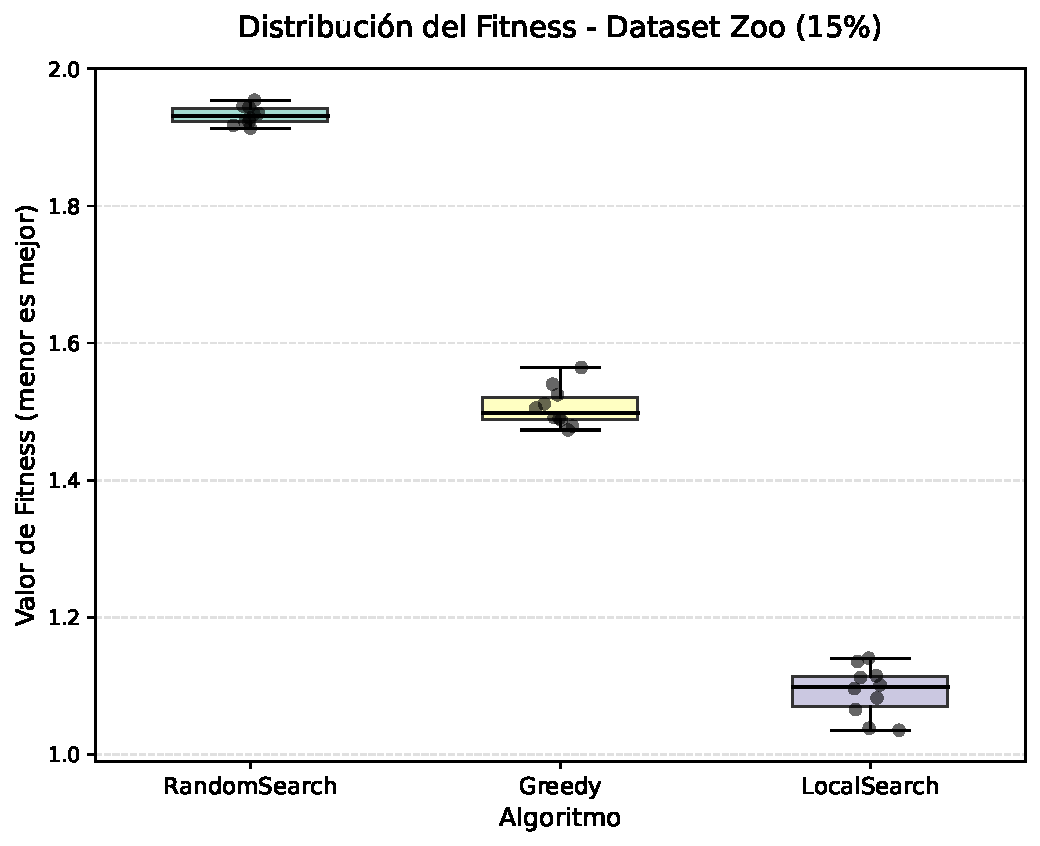
\includegraphics[width=\textwidth]{graficos/boxplot_zoo_15.pdf}
            \caption{15\% de restricciones}
            \label{fig:boxplot_zoo_15}
        \end{subfigure}\hfill
        \begin{subfigure}{0.49\textwidth}
            \centering
            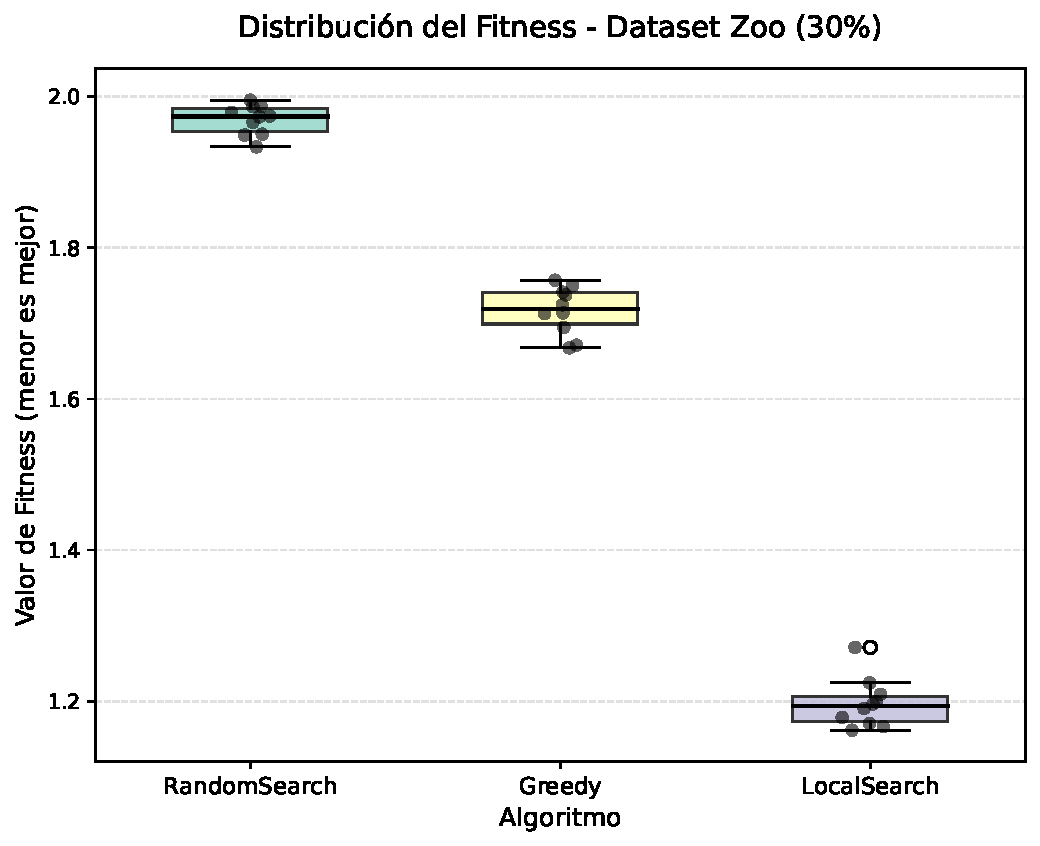
\includegraphics[width=\textwidth]{graficos/boxplot_zoo_30.pdf}
            \caption{30\% de restricciones}
            \label{fig:boxplot_zoo_30}
        \end{subfigure}
        \caption{Distribución de los valores de Fitness obtenidos para el dataset \textbf{Zoo} en 10 ejecuciones independientes.}
        \label{fig:boxplot_zoo}
    \end{figure}

    \begin{figure}[H]
        \centering
        \begin{subfigure}{0.49\textwidth}
            \centering
            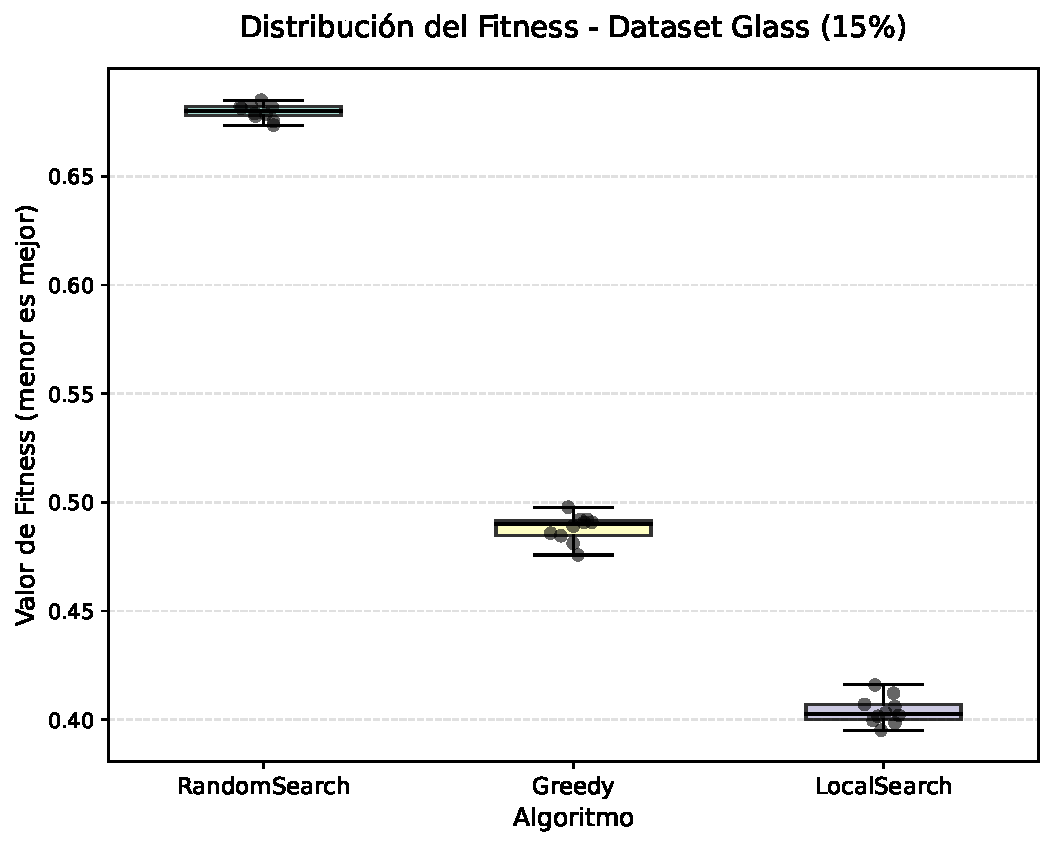
\includegraphics[width=\textwidth]{graficos/boxplot_glass_15.pdf}
            \caption{15\% de restricciones}
            \label{fig:boxplot_glass_15}
        \end{subfigure}\hfill
        \begin{subfigure}{0.49\textwidth}
            \centering
            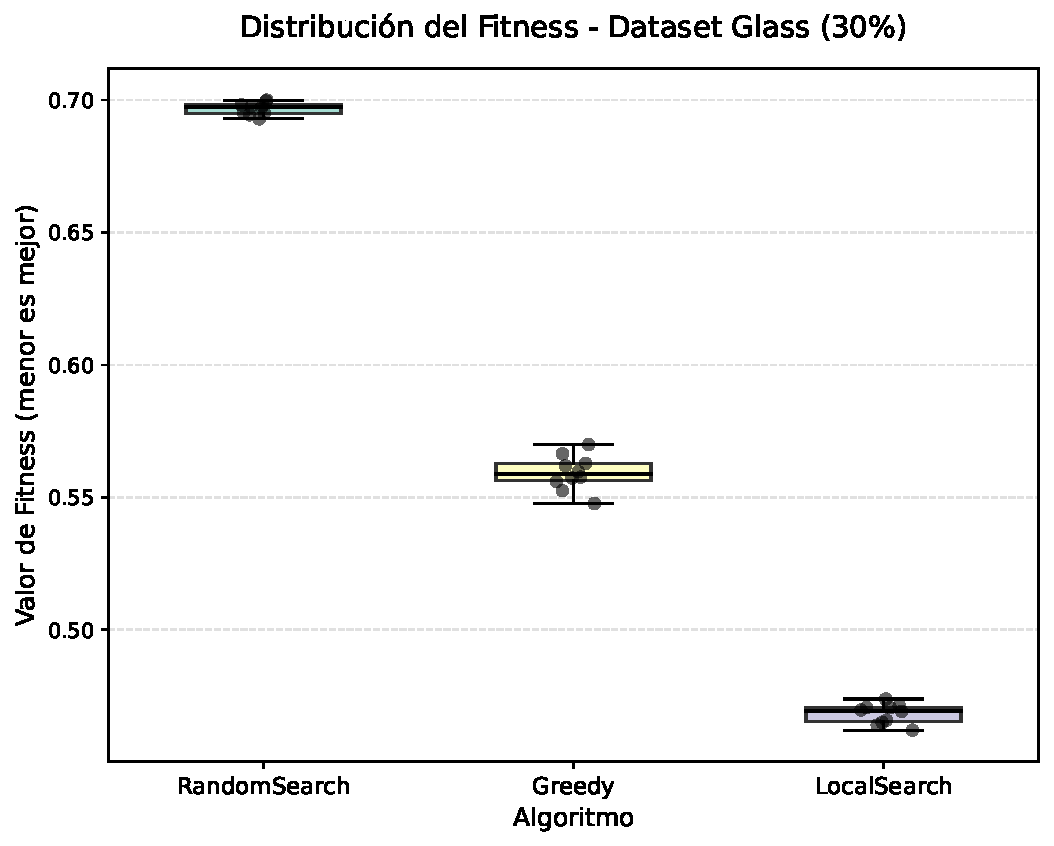
\includegraphics[width=\textwidth]{graficos/boxplot_glass_30.pdf}
            \caption{30\% de restricciones}
            \label{fig:boxplot_glass_30}
        \end{subfigure}
        \caption{Distribución de los valores de Fitness obtenidos para el dataset \textbf{Glass} en 10 ejecuciones independientes.}
        \label{fig:boxplot_glass}
    \end{figure}

    \begin{figure}[H]
        \centering
        \begin{subfigure}{0.49\textwidth}
            \centering
            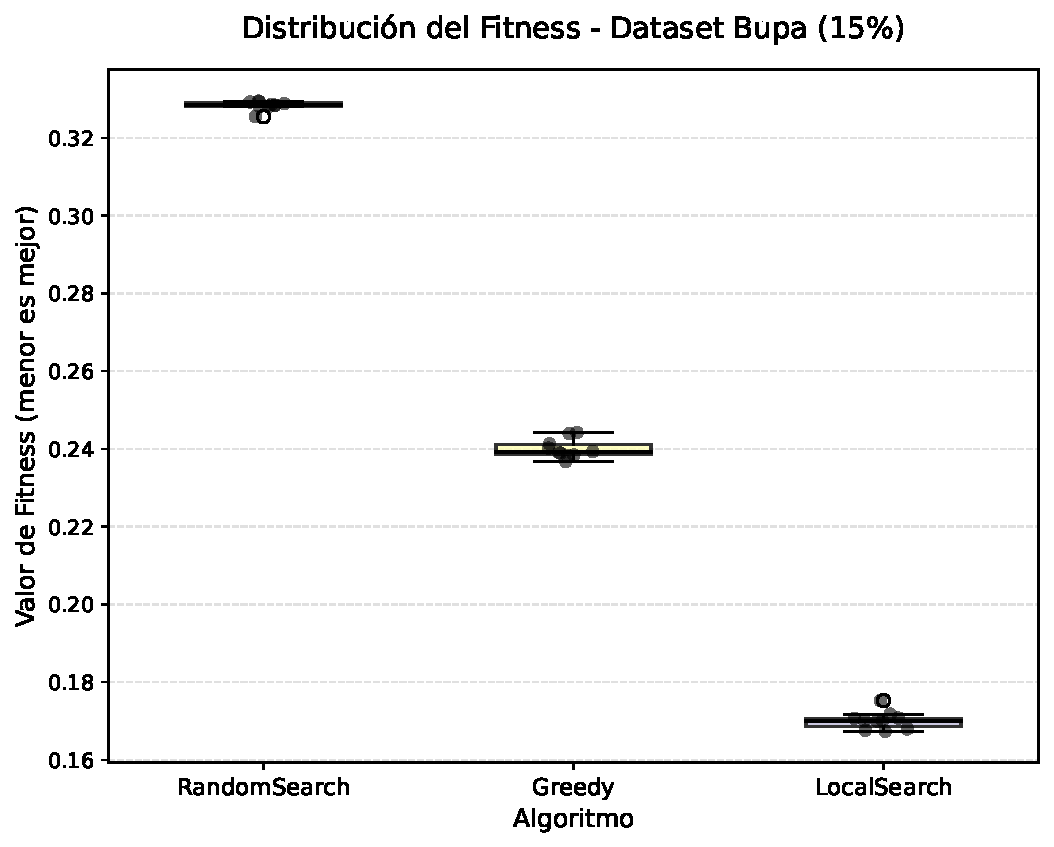
\includegraphics[width=\textwidth]{graficos/boxplot_bupa_15.pdf}
            \caption{15\% de restricciones}
            \label{fig:boxplot_bupa_15}
        \end{subfigure}\hfill
        \begin{subfigure}{0.49\textwidth}
            \centering
            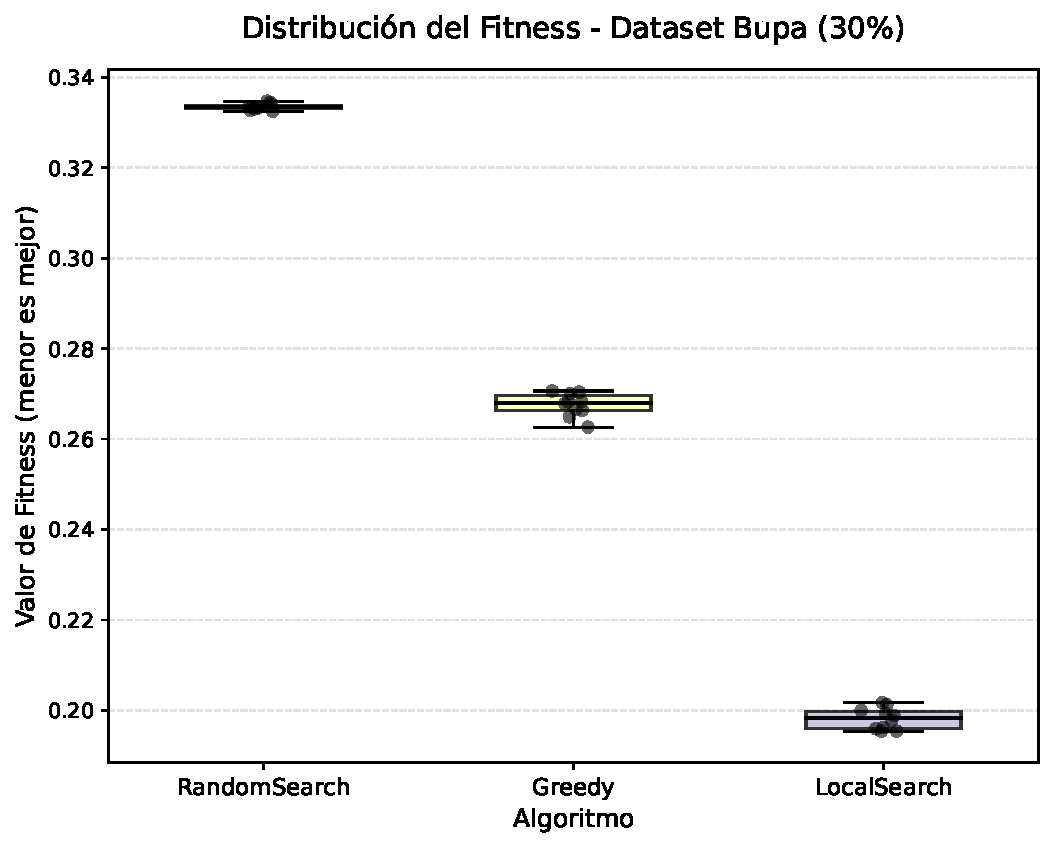
\includegraphics[width=\textwidth]{graficos/boxplot_bupa_30.pdf}
            \caption{30\% de restricciones}
            \label{fig:boxplot_bupa_30}
        \end{subfigure}
        \caption{Distribución de los valores de Fitness obtenidos para el dataset \textbf{Bupa} en 10 ejecuciones independientes.}
        \label{fig:boxplot_bupa}
    \end{figure}

    \subsection{Análisis de resultados}

    A partir de las métricas obtenidas en las tablas globales y la observación de la distribución en las gráficas, se pueden extraer conclusiones muy claras sobre el rendimiento y comportamiento de los tres algoritmos evaluados. El análisis se dividirá en cuatro bloques principales: calidad de las soluciones, satisfacción de restricciones, eficiencia computacional y el impacto de la complejidad del problema.

    \subsubsection{Calidad de las soluciones}
    Comparando los resultados llegamos a las siguientes conclusiones de cada algoritmo:
    
    \begin{itemize}
        \item \textbf{Búsqueda Local (BL):} Ha demostrado ser el algoritmo más robusto y eficaz en términos de calidad pura. Para todos los conjuntos de datos (Zoo, Glass y Bupa) y ratios de restricción, la BL obtiene consistentemente los valores más bajos tanto de fitness general como de distancia intra-clúster. Esto demuestra que la exploración del vecindario guiada por gradiente descendente permite refinar adecuadamente las asignaciones hasta alcanzar mínimos locales de muy buena calidad.
        \item \textbf{Greedy:} Se posiciona como una heurística intermedia. Supera ampliamente al modelo aleatorio, logrando configuraciones razonablemente buenas, pero se estanca en óptimos locales peores que los de la Búsqueda Local, ya que su enfoque constructivo no le permite retroceder o reevaluar asignaciones previas.
        \item \textbf{Algoritmo Aleatorio:} Como era de esperar en espacios de búsqueda combinatorios tan amplios, el muestreo aleatorio puro (incluso con 100.000 iteraciones) ofrece resultados no tan satisfactorios. Presenta la mayor dispersión y los peores valores de \textit{fitness} (nos sirve para ver que efectivamente los otros algoritmos funcionan bien).
    \end{itemize}

    \subsubsection{Satisfacción de restricciones}
    Si estudiamos el número de restricciones incumplidas llegamos a que:
    
    \begin{itemize}
        \item El algoritmo \textbf{Greedy} es el claro ganador en el cumplimiento de las restricciones (valores más cercanos a 0 en todas las configuraciones). Al evaluar de manera determinista la violación exacta en cada inserción, el algoritmo logra evitar casi por completo incumplir las restricciones
        \item Por el contrario, la \textbf{Búsqueda Local} sacrifica este factor. Dado que la función objetivo pondera la distancia y las restricciones mediante el parámetro $\lambda$, la BL encuentra que, en ciertas ocasiones, es mejor (globalmente) violar una restricción para agrupar elementos geométricamente muy cercanos, reduciendo la distancia a cambio de una pequeña penalización en la infactibilidad.
    \end{itemize}

    \subsubsection{Eficiencia computacional}
    El análisis del eficiencia computacional también es interesante:
    
    \begin{itemize}
        \item \textbf{Aleatorio vs. Búsqueda Local:} El algoritmo Aleatorio consume siempre el máximo de evaluaciones (100.000) de forma bruta. Esto se traduce en tiempos altos (ej. hasta 2823 ms en Bupa 30\%). Por su parte, la BL realiza un número variable de evaluaciones hasta converger (entre 6.200 en Zoo y 82.000 en Bupa). Sin embargo, gracias a la evaluación factorizada, los tiempos de la BL son sistemáticamente inferiores a los del algoritmo aleatorio (ej. 1310 ms en Bupa 30\%), demostrando que el diseño de estructuras de datos eficientes compensa con creces el coste de generar vecindarios.
        \item \textbf{Greedy:} Es indiscutiblemente el algoritmo más rápido en términos absolutos ya que construye la solución en una sola pasada (registrando una única evaluación en cada caso).
    \end{itemize}

    \subsubsection{Impacto de la escalabilidad y las restricciones}
    Finalmente, los experimentos evidencian la sensibilidad de los algoritmos ante el aumento de la complejidad:
    
    \begin{itemize}
        \item \textbf{Aumento del Ratio de Restricciones (15\% a 30\%):} Al duplicar las imposiciones sobre el espacio geométrico, la dificultad del problema aumenta de forma evidente. En los tres datasets se observa que pasar al 30\% provoca un empeoramiento del fitness global, un incremento en la tasa de incumplimiento y un ligero aumento en los tiempos de ejecución.
        \item \textbf{Tamaño del Dataset:} Al transicionar de Zoo (101 instancias) a Glass (214) y Bupa (345), el tiempo de ejecución crece bastante (especialmente de Glass a Bupa, donde también pasamos de $k=7$ a $k=16$). La Búsqueda Local requiere explorar vecindarios mucho más grandes, aumentando sus tiempos y las evaluaciones requeridas para llegar a un óptimo local (de unas 6.000 en Zoo a más de 80.000 en Bupa).
    \end{itemize}

    \textbf{Conclusión general:} La \textbf{Búsqueda Local} con evaluación factorizada es sin ninguna duda el mejor método para este problema. Consigue el mejor equilibrio entre cercanía de los puntos de los clústeres, tolerancia al cumplimiento de restricciones y eficiencia temporal. El algoritmo \textbf{Greedy} podría servir de semilla inicial para algoritmos más complejos, dada su alta rapidez y factibilidad.

\end{document}